% !TEX root = ../main.tex

\section{Model development}

Details about the biomass pyrolysis kinetics, biomass characterization method, and computational models developed for the entrained flow reactor are discussed in the following sections.

\subsection{Biomass pyrolysis kinetics}

The kinetic reaction mechanisms presented in the Debiagi et al. 2018 paper \cite{Debiagi-2018} are used to model biomass pyrolysis in the entrained flow reactor. Table \ref{tab:chem-kinetics} summarizes the reactions along with the associated prefactors and activation energies. A description of the chemical species in the Debiagi et al. kinetic scheme is provided in Table \ref{tab:chem-species}. Species are grouped into solid, metaplastic, gas, and liquid phases. Solid and metaplastic species are combined and compared to the EFR char yield. All liquid species are combined and compared to the EFR total liquid yield.

\begin{center}
    \footnotesize
    \setlength\LTleft{-1in}
    \setlength\LTright{-1in}
    \begin{longtable}{cp{4in}lr}
        \caption{Kinetic reactions for biomass pyrolysis where A is the prefactor, E is the activation energy, and T is temperature. Source \cite{Debiagi-2018}.}
        \label{tab:chem-kinetics} \\
        \toprule
        Item & Reaction & A (1/s) & E (cal/mol) \\
        \midrule
        1  & CELL $\rightarrow$ CELLA & 1.5 $\times$ 10$^{14}$ & 47,000 \\
        2  & CELLA $\rightarrow$ 0.40 CH2OHCHO + 0.03 CHOCHO + 0.17 CH3CHO + 0.25 C6H6O3 + 0.35 C2H5CHO + 0.20 CH3OH + 0.15 CH2O + 0.49 CO + 0.05 G\{CO\} + 0.43 CO2 + 0.13 H2 + 0.93 H2O + 0.05 G\{COH2\} loose + 0.02 HCOOH + 0.05 CH2OHCH2CHO + 0.05 CH4 + 0.1 G\{H2\} + 0.66 CHAR & 2.5 $\times$ 10$^6$ & 19,100 \\
        3  & CELLA $\rightarrow$ C6H10O5 & 3.3 $\times$ T & 10,000 \\
        4  & CELL $\rightarrow$ 4.45 H2O + 5.45 CHAR + 0.12 G\{COH2\} stiff + 0.18 G\{COH2\} loose + 0.25 G\{CO\} + 0.125 G\{H2\} + 0.125 H2 & 9.0 $\times$ 10$^7$ & 31,000 \\
        5  & GMSW $\rightarrow$ 0.70 HCE1 + 0.30 HCE2 & 1.0 $\times$ 10$^{10}$ & 31,000 \\
        6  & XYHW $\rightarrow$ 0.35 HCE1 + 0.65 HCE2 & 1.25 $\times$ 10$^{11}$ & 31,400 \\
        7  & XYGR $\rightarrow$ 0.12 HCE1 + 0.88 HCE2 & 1.25 $\times$ 10$^{11}$ & 30,000 \\
        8  & HCE1 $\rightarrow$ 0.25 C5H8O4 + 0.25 C6H10O5 + 0.16 FURFURAL + 0.13 C6H6O3 + 0.09 CO2 + 0.1 CH4 + 0.54 H2O + 0.06 CH2OHCH2CHO + 0.1 CHOCHO + 0.02 H2 + 0.1 CHAR & 16.0 $\times$ T & 12,900 \\
        9  & HCE1 $\rightarrow$ 0.4 H2O + 0.39 CO2 + 0.05 HCOOH + 0.49 CO + 0.01 G\{CO\} + 0.51 G\{CO2\} + 0.05 G\{H2\} + 0.4 CH2O + 0.43 G\{COH2\} loose + 0.3 CH4 + 0.325 G\{CH4\} + 0.1 C2H4 + 0.075 G\{C2H4\} + 0.975 CHAR + 0.37 G\{COH2\} stiff + 0.1 H2 + 0.2 G\{C2H6\} & 3.0 $\times$ 10$^{-3}$ $\times$ T & 3,600 \\
        10 & HCE2 $\rightarrow$ 0.3 CO + 0.5125 CO2 + 0.1895 CH4 + 0.5505 H2 + 0.056 H2O + 0.049 C2H5OH + 0.035 CH2OHCHO + 0.105 CH3CO2H + 0.0175 HCOOH + 0.145 FURFURAL + 0.05 G\{CH4\} + 0.105 G\{CH3OH\} + 0.1 G\{C2H4\} + 0.45 G\{CO2\} + 0.18 G\{COH2\} loose + 0.7125 CHAR + 0.21 G\{H2\} + 0.78 G\{COH2\} stiff + 0.2 G\{C2H6\} & 7.0 $\times$ 10$^9$ & 30,500 \\
        11 & LIGH $\rightarrow$ LIGOH + 0.5 C2H5CHO + 0.4 C2H4 + 0.2 CH2OHCHO + 0.1 CO + 0.1 C2H6 & 6.7 $\times$ 10$^{12}$ & 37,500 \\
        12 & LIGO $\rightarrow$ LIGOH + CO2 & 3.3 $\times$ 10$^8$ & 25,500 \\
        13 & LIGC $\rightarrow$ 0.35 LIGCC + 0.1 VANILLIN + 0.1 C6H5OCH3 + 0.27 C2H4 + H2O + 0.17 G\{COH2\} loose + 0.4 G\{COH2\} stiff + 0.22 CH2O + 0.21 CO + 0.1 CO2 + 0.36 G\{CH4\} + 5.85 CHAR + 0.2 G\{C2H6\} + 0.1 G\{H2\} & 1.0 $\times$ 10$^{11}$ & 37,200 \\
        14 & LIGCC $\rightarrow$ 0.25 VANILLIN + 0.15 CRESOL + 0.15 C6H5OCH3 + 0.35 CH2OHCHO + 0.7 H2O + 0.45 CH4 + 0.3 C2H4 + 0.7 H2 + 1.15 CO + 0.4 G\{CO\} + 6.80 CHAR + 0.4 C2H6 & 1.0 $\times$ 10$^4$ & 24,800 \\
        15 & LIGOH $\rightarrow$ 0.9 LIG + H2O + 0.1 CH4 + 0.6 CH3OH + 0.3 G\{CH3OH\} + 0.05 CO2 + 0.65 CO + 0.6 G\{CO\} + 0.05 HCOOH + 0.45 G\{COH2\} loose + 0.4 G\{COH2\} stiff + 0.25 G\{CH4\} + 0.1 G\{C2H4\} + 0.15 G\{C2H6\} + 4.25 CHAR + 0.025 C24H28O4 + 0.1 C2H3CHO & 1.5 $\times$ 10$^8$ & 30,000 \\
        16 & LIG $\rightarrow$ VANILLIN + 0.1 C6H5OCH3 + 0.5 C2H4 + 0.6 CO + 0.3 CH3CHO + 0.1 CHAR & 4.0 $\times$ T & 12,000 \\
        17 & LIG $\rightarrow$ 0.6 H2O + 0.3 CO + 0.1 CO2 + 0.2 CH4 + 0.4 CH2O + 0.2 G\{CO\} + 0.4 G\{CH4\} + 0.5 G\{C2H4\} + 0.4 G\{CH3OH\} + 1.25 G\{COH2\} loose + 0.65 G\{COH2\} stiff + 6.1 CHAR + 0.1 G\{H2\} & 8.3 $\times$ 10$^{-2}$ $\times$ T & 8,000 \\
        18 & LIG $\rightarrow$ 0.6 H2O + 2.6 CO + 0.6 CH4 + 0.4 CH2O + 0.75 C2H4 + 0.4 CH3OH + 4.5 CHAR + 0.5 C2H6 & 1.5 $\times$ 10$^9$ & 31,500 \\
        19 & TGL $\rightarrow$ C2H3CHO + 2.5 MLINO + 0.5 U2ME12 & 7.0 $\times$ 10$^{12}$ & 45,700 \\
        20 & TANN $\rightarrow$ 0.85 C6H5OH + 0.15 G\{C6H5OH\} + G\{CO\} + H2O + ITANN & 2.0 $\times$ 10$^1$ & 10,000 \\
        21 & ITANN $\rightarrow$ 5 CHAR + 2 CO + H2O + 0.55 G\{COH2\} loose + 0.45 G\{COH2\} stiff & 1.0 $\times$ 10$^3$ & 25,000 \\
        22 & G\{CO2\} $\rightarrow$ CO2 & 1.0 $\times$ 10$^6$ & 24,500 \\
        23 & G\{CO\} $\rightarrow$ CO & 5.0 $\times$ 10$^{12}$ & 52,500 \\
        24 & G\{CH3OH\} $\rightarrow$ CH3OH & 2.0 $\times$ 10$^{12}$ & 50,000 \\
        25 & G\{COH2\}loose $\rightarrow$ 0.2 CO + 0.2 H2 + 0.8 H2O + 0.8 CHAR & 6.0 $\times$ 10$^{10}$ & 50,000 \\
        26 & G\{C2H6\} $\rightarrow$ C2H6 & 1.0 $\times$ 10$^{11}$ & 52,000 \\
        27 & G\{CH4\} $\rightarrow$ CH4 & 1.0 $\times$ 10$^{11}$ & 53,000 \\
        28 & G\{C2H4\} $\rightarrow$ C2H4 & 1.0 $\times$ 10$^{11}$ & 54,000 \\
        29 & G\{C6H5OH\} $\rightarrow$ C6H5OH & 1.5 $\times$ 10$^{12}$ & 55,000 \\
        30 & G\{COH2\}stiff $\rightarrow$ 0.8 CO + 0.8 H2 + 0.2 H2O + 0.2 CHAR & 1.0 $\times$ 10$^9$ & 59,000 \\
        31 & G\{H2\} $\rightarrow$ H2 & 1.0 $\times$ 10$^8$ & 70,000 \\
        32 & ACQUA $\rightarrow$ H2O & 1.0 $\times$ T & 8,000 \\
        \bottomrule
    \end{longtable}
\end{center}

\begin{center}
    \footnotesize
    \begin{longtable}{cllll}
        \caption{Description of the chemical species in the Debiagi kinetics scheme for biomass pyrolysis. Source \cite{Debiagi-2018}.}
        \label{tab:chem-species} \\
        \toprule
        Item & Name & Formula & Phase & Description \\
        \midrule
        1  & CELL           & C$_6$H$_{10}$O$_5$      & \cellcolor{green!25}solid        & cellulose \\
        2  & CELLA          & C$_6$H$_{10}$O$_5$      & \cellcolor{green!25}solid        & active cellulose \\
        3  & GMSW           & C$_5$H$_{8}$O$_4$       & \cellcolor{green!25}solid        & hemicellulose softwood \\
        4  & XYHW           & C$_5$H$_{8}$O$_4$       & \cellcolor{green!25}solid        & hemicellulose hardwood \\
        5  & XYGR           & C$_5$H$_{8}$O$_4$       & \cellcolor{green!25}solid        & hemicellulose grass \\
        6  & HCE1           & C$_5$H$_{8}$O$_4$       & \cellcolor{green!25}solid        & intermediate hemicellulose \\
        7  & HCE2           & C$_5$H$_{8}$O$_4$       & \cellcolor{green!25}solid        & intermediate hemicellulose \\
        8  & ITANN          & C$_8$H$_{4}$O$_4$       & \cellcolor{green!25}solid        & intermediate phenolics \\
        9  & LIG            & C$_{11}$H$_{12}$O$_4$   & \cellcolor{green!25}solid        & intermediate lignin \\
        10 & LIGC           & C$_{15}$H$_{14}$O$_4$   & \cellcolor{green!25}solid        & carbon rich lignin \\
        11 & LIGCC          & C$_{15}$H$_{14}$O$_4$   & \cellcolor{green!25}solid        & intermediate lignin \\
        12 & LIGH           & C$_{22}$H$_{28}$O$_9$   & \cellcolor{green!25}solid        & hydrogen rich lignin \\
        13 & LIGO           & C$_{20}$H$_{22}$O$_{10}$& \cellcolor{green!25}solid        & oxygen rich lignin \\
        14 & LIGOH          & C$_{19}$H$_{22}$O$_8$   & \cellcolor{green!25}solid        & intermediate lignin \\
        15 & TANN           & C$_{15}$H$_{12}$O$_7$   & \cellcolor{green!25}solid        & tannins \\
        16 & TGL            & C$_{57}$H$_{100}$O$_7$  & \cellcolor{green!25}solid        & triglycerides \\
        17 & CHAR           & C                       & \cellcolor{green!25}solid        & char as pure carbon \\
        18 & ACQUA          & H$_2$O                  & \cellcolor{green!25}solid        & biomass moisture content \\
        19 & G\{COH2\} loose& CH$_2$O                 & \cellcolor{orange!25}metaplastic & loose formaldehyde \\
        20 & G\{CO2\}       & CO$_2$                  & \cellcolor{orange!25}metaplastic & trapped carbon dioxide \\
        21 & G\{CO\}        & CO                      & \cellcolor{orange!25}metaplastic & trapped carbon monoxide \\
        22 & G\{CH3OH\}     & CH$_4$O                 & \cellcolor{orange!25}metaplastic & trapped methanol \\
        23 & G\{CH4\}       & CH$_4$                  & \cellcolor{orange!25}metaplastic & trapped methane \\
        24 & G\{C2H4\}      & C$_2$H$_4$              & \cellcolor{orange!25}metaplastic & trapped ethylene \\
        25 & G\{C6H5OH\}    & C$_6$H$_6$O             & \cellcolor{orange!25}metaplastic & trapped phenol \\
        26 & G\{COH2\} stiff& CH$_2$O                 & \cellcolor{orange!25}metaplastic & stiff formaldehyde \\
        27 & G\{H2\}        & H$_2$                   & \cellcolor{orange!25}metaplastic & trapped hydrogen \\
        28 & G\{C2H6\}      & C$_2$H$_6$              & \cellcolor{orange!25}metaplastic & trapped ethane \\
        29 & C2H4           & C$_2$H$_4$              & \cellcolor{purple!25}gas         & ethylene \\
        30 & C2H6           & C$_2$H$_6$              & \cellcolor{purple!25}gas         & ethane \\
        31 & CH2O           & CH$_2$O                 & \cellcolor{purple!25}gas         & formaldehyde \\
        32 & CH4            & CH$_4$                  & \cellcolor{purple!25}gas         & methane \\
        33 & CO             & CO                      & \cellcolor{purple!25}gas         & carbon monoxide \\
        34 & CO2            & CO$_2$                  & \cellcolor{purple!25}gas         & carbon dioxide \\
        35 & H2             & H$_2$                   & \cellcolor{purple!25}gas         & hydrogen \\
        36 & C2H3CHO        & C$_3$H$_4$O             & \cellcolor{blue!25}liquid        & acrolein \\
        37 & C2H5CHO        & C$_3$H$_6$O             & \cellcolor{blue!25}liquid        & propionaldehyde \\
        38 & C2H5OH         & C$_2$H$_6$O             & \cellcolor{blue!25}liquid        & ethanol \\
        39 & C5H8O4         & C$_5$H$_8$O$_4$         & \cellcolor{blue!25}liquid        & xylofuranose \\
        40 & C6H10O5        & C$_6$H$_{10}$O$_5$      & \cellcolor{blue!25}liquid        & levoglucosan \\
        41 & C6H5OCH3       & C$_7$H$_8$O             & \cellcolor{blue!25}liquid        & anisole \\
        42 & C6H5OH         & C$_6$H$_6$O             & \cellcolor{blue!25}liquid        & phenol \\
        43 & C6H6O3         & C$_6$H$_6$O$_3$         & \cellcolor{blue!25}liquid        & hydroxymethylfurfural \\
        44 & C24H28O4       & C$_{24}$H$_{28}$O$_4$   & \cellcolor{blue!25}liquid        & heavy molecular weight lignin \\
        45 & CH2OHCH2CHO    & C$_3$H$_6$O$_2$         & \cellcolor{blue!25}liquid        & propionic acid \\
        46 & CH2OHCHO       & C$_2$H$_4$O$_2$         & \cellcolor{blue!25}liquid        & acetic acid \\
        47 & CH3CHO         & C$_2$H$_4$O             & \cellcolor{blue!25}liquid        & acetaldehyde \\
        48 & CH3CO2H        & C$_2$H$_4$O$_2$         & \cellcolor{blue!25}liquid        & acetic acid \\
        49 & CH3OH          & CH$_4$O                 & \cellcolor{blue!25}liquid        & methanol \\
        50 & CHOCHO         & C$_2$H$_2$O$_2$         & \cellcolor{blue!25}liquid        & glyoxal \\
        51 & CRESOL         & C$_7$H$_8$O             & \cellcolor{blue!25}liquid        & cresol \\
        52 & FURFURAL       & C$_5$H$_4$O$_2$         & \cellcolor{blue!25}liquid        & 2-furaldehyde \\
        53 & H2O            & H$_2$O                  & \cellcolor{blue!25}liquid        & water from reactions \\
        54 & HCOOH          & CH$_2$O$_2$             & \cellcolor{blue!25}liquid        & formic acid \\
        55 & MLINO          & C$_{19}$H$_{34}$O$_2$   & \cellcolor{blue!25}liquid        & methyl linoleate \\
        56 & U2ME12         & C$_{13}$H$_{22}$O$_2$   & \cellcolor{blue!25}liquid        & linalyl propionate \\
        57 & VANILLIN       & C$_8$H$_8$O$_3$         & \cellcolor{blue!25}liquid        & vanillin \\
        \bottomrule
    \end{longtable}
\end{center}

\subsection{Biomass characterization}

The Debiagi kinetics rely on an initial biomass composition defined as cellulolose, hemicellulose, lignin-c, lignin-h, lignin-o, tannins, and triglycerides. According to the Debiagi et al. 2015 paper \cite{Debiagi-2015}, the chemical components of the biomass are defined as shown below in Table \ref{tab:chem-components}. The Debiagi article does not provide information on how to experimentally determine these components; therefore, the reader must decide on appropriate measurement techniques.

\begin{table}[H]
    \centering
    \caption{Chemical components of biomass according to Debiagi et al. \cite{Debiagi-2015}.}
    \label{tab:chem-components}
    \begin{tabular}{lp{2.2in}}
        \toprule
        Biomass composition & Description \\
        \midrule
        cellulose     & glucan \\
        \addlinespace[0.1in]
        hemicellulose & mixture of sugars such as hexoses and pentoses; mainly xylose, mannose, galactose, and arabinose \\
        \addlinespace[0.1in]
        lignin        & aromatic alcohols such as coniferyl, sinapyl, p-coumaryl alcohol \\
        \addlinespace[0.1in]
        lignin-c      & carbon-rich lignin \\
        \addlinespace[0.1in]
        lignin-h      & hydrogen-rich lignin \\
        \addlinespace[0.1in]
        lignin-o      & oxygen-rich lignin \\
        \addlinespace[0.1in]
        tannins       & hydrophilic extractives, phenolics, ethanol and water, represented by a gallocatechin polymer \\
        \addlinespace[0.1in]
        triglycerides & hydrophobic extractives, hexane and ether, linoleic acid \\
        \bottomrule
    \end{tabular}
\end{table}

Ideally, the composition of the biomass would be directly measured; otherwise, the characterization method discussed in the Debiagi paper estimates the composition based on elemental analysis data \cite{Debiagi-2015}. The characterization method utilizes carbon and hydrogen obtained from elemental (ultimate) analysis of the biomass to predict the biochemical composition in terms of cellulose, hemicellulose, and lignin. Splitting parameters $\alpha$, $\beta$, $\gamma$, $\delta$, $\epsilon$ are used to improve the validity of the characterization procedure by accounting for extractives in the biomass.

\subsection{Batch reactor model}

The material balance for a typical chemical reactor is shown in Equation \ref{eq:typical-balance} where $C_0$ is inlet concentration, $C$ is outlet concentration, $v$ is volumetric flow rate, $r$ is the reaction rate, and $V$ is the reactor volume.

\begin{equation}
    \label{eq:typical-balance}
    \begin{aligned}
        accumulation &= input - output + reaction \\
        \frac{dC}{dt} V &= v C_0 - v C + r V
    \end{aligned}
\end{equation}

A batch reactor was modeled to understand the time scales associated with the biomass pyrolysis kinetics. For the batch reactor, input and output is zero therefore only the accumulation and reaction terms remain in the material balance. For a constant volume reactor the $V$ terms cancel out; therefore, Equation \ref{eq:batch-balance} represents the material balance for a batch reactor model. A depiction of a batch reactor can be seen in Figure \ref{fig:batch-reactor}. The Cantera Python package was used to model the batch reactor as an IdealGasReactor \cite{Cantera-2018}.

\begin{equation}
    \label{eq:batch-balance}
    \begin{aligned}
        accumulation &= 0 - 0 + reaction \\
        \frac{dC}{dt} &= r
    \end{aligned}
\end{equation}

\begin{figure}[H]
    \centering
    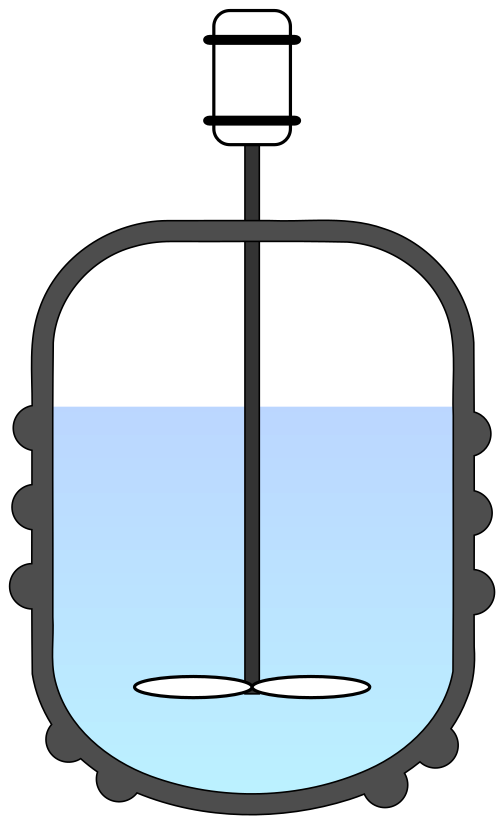
\includegraphics[width=0.2\textwidth]{figures/batch-reactor.png}
    \caption{Representation of a batch reactor system. Source: Wikipedia.}
    \label{fig:batch-reactor}
\end{figure}

\subsection{Sensitivity analysis}

A sensitivity analysis was performed with a batch reactor model using the Debiagi pyrolysis kinetics. The awesome SALib Python package was implemented for sample generation and calculation of the Sobol indices \cite{Herman-2017}. The first-order index (S1) measures the contribution of a single model input to the variance of the model output. The total-order index (ST) measures higher-order contributions of the model input to the output variance.

An overview of the steps used to determine the Sobol sensitivity indices is shown in Figure \ref{fig:sa-diagram}. A sample represents a biomass composition in terms of cellulose, hemicellulose, lignin-c, lignin-h, lignin-o, tannins, and triglycerides; this sample is the model input for the batch reactor. The Saltelli method provided by the SALib package was used to generate a large number of samples for the Sobol sensitivity analysis. Each sample was normalized such that the mass fraction of the biomass composition components added up to one. All of the samples (biomass compositions) were utilized in a batch reactor model where the final concentrations were used for the Sobol sensitivity analysis.

\begin{figure}[H]
    \centering
    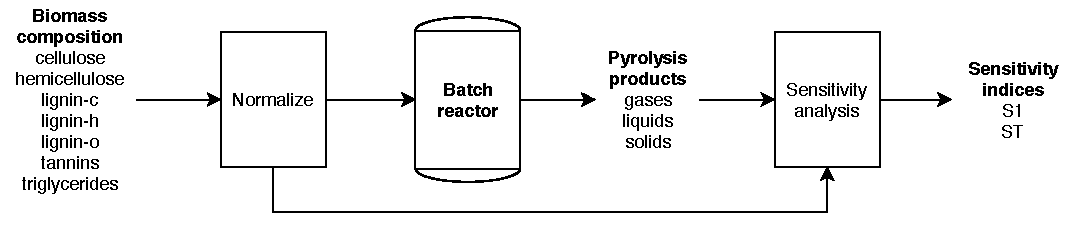
\includegraphics[width=\textwidth]{figures/sa-diagram.pdf}
    \caption{Steps for performing a sensitivity analysis of the Debiagi kinetics with a batch reactor model.}
    \label{fig:sa-diagram}
\end{figure}

\subsection{Reduced-order model}

The entrained flow reactor is essentially a long pipe that conveys biomass particles from one end to the other. The EFR is modeled as a plug flow reactor (PFR) which is represented as a series of continuously stirred tank reactors (CSTRs). A mixer model combines the nitrogen gas and biomass streams into one stream for the CSTR model. The number of CSTRs needed for the model is determined by the final product yield. When the final yield no longer changes with the number of CSTRs, then that number is considered a reasonable approximation of the PFR. An example of this reduced-order modeling technique is shown in Figure \ref{fig:pfr-diagram}. As with the batch reactor model, the Cantera Python package was used to model the series of CSTRs as a chain of IdealGasConstPressureReactor \cite{Cantera-2018}.

\begin{figure}[H]
    \centering
    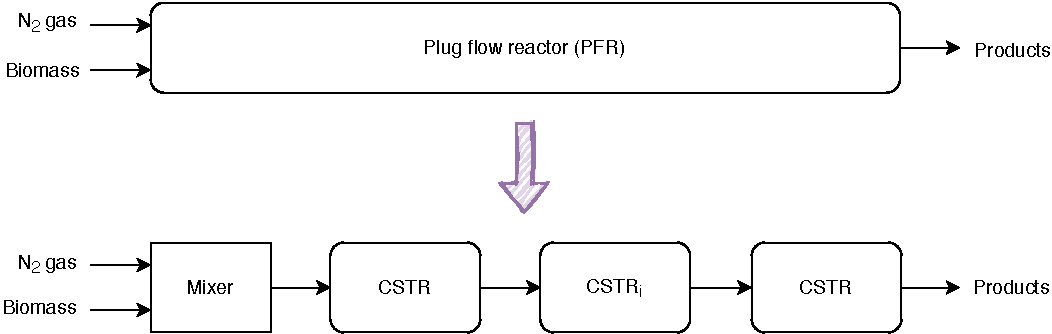
\includegraphics[width=\textwidth]{figures/pfr-diagram.pdf}
    \caption{Depiction of the entrained flow reactor modeled as a PFR which is represented my a mixer and series $i$ of CSTRs.}
    \label{fig:pfr-diagram}
\end{figure}
